\documentclass{beamer}

\hypersetup{pdfpagemode=FullScreen}

\usepackage[utf8]{inputenc}
\usepackage{default}
\usepackage[italian]{babel}
\usepackage{amsmath}
\usepackage{amsfonts}
\usepackage{xfrac}
\usepackage{tabularx}
\usepackage{graphicx}
\graphicspath{{img/}}

\usepackage{subcaption}
\captionsetup{compatibility=false}

\newcommand{\der}[2]{\frac{\partial #1}{\partial #2}}
\newcommand{\dder}[2]{\frac{\partial^2 #1}{\partial #2^2}}
\newcommand{\dmix}[3]{\frac{\partial^2 #1}{\partial #2 \partial #3}}

\AtBeginSection[]
{
  \begin{frame}
    \frametitle{Indice}
    \tableofcontents[currentsection]
  \end{frame}
}

%%presentation theme
\usetheme{Warsaw}

%%remove navigation symbols
\beamertemplatenavigationsymbolsempty

%%add page numbering
\useoutertheme{infolines}
% \setbeamertemplate{footline}


\title[PIDE pricing con elementi finiti] % (optional, only for long titles)
{Metodo a elementi finiti per il pricing di opzioni multi-asset con modelli di L\'evy}
\subtitle{Progetto di Programmazione Avanzata per il Calcolo Scientifico}
\author[Foresta, Re] % (optional, for multiple authors)
{Nahuel~Foresta \and Giorgio G.~Re}
\institute[Politecnico di Milano]{Dipartimento di Matematica\\ \bf{Politecnico di Milano}} % (optional)
\date{\today}





\begin{document}


%%%%%%%%%%%%%%%%%%%%%%%%%%%%%%%%%%%%%%%%%%%%%%%%%%%%%%%%%%%%%%%%%%%%%%%%%%%%%%%%%%%%%%%%%%%%%%%%%%%%%%%%%%%%%%%%%%%%%%%%%%%%%%%%%%%%%%%%%%%%%%%%%%%%%%%%%%%%%%%%%%%%%%%%%%%%%%%%%%%%%%%%%%%%%%%%%%%%%%%%%%%%%%%%%%%%%%%%%%%%%%%%%%%%%%%%%%%%%%%%%%%%%%%%%%%%%%%%%%

\begin{frame}
\centering
 
\includegraphics[scale=0.2]{poli_logo}
 \maketitle
\end{frame}



%%%%%%%%%%%%%%%%%%%%%%%%%%%%%%%%%%%%%%%%%%%%%%%%%%%%%%%%%%%%%%%%%%%%%%%%%%%%%%%%%%%%%%%%%%%%%%%%%%%%%%%%%%%%%%%%%%%%%%%%%%%%%%%%%
\section{Introduzione}
\begin{frame}
\frametitle{Il progetto}
\begin{block}{Scopo}
Lo scopo di questo progetto è creare una piccola libreria per il \emph{pricing} di derivati finanziari con il metodo degli elementi finiti, utilizzando la libreria \textsf{deal.ii}.
L'idea è che l'utente possa sia utilizzare gli strumenti presenti, sia aggiungerne altri nel caso di bisogno, con grande facilità (ereditariet\`a).
\end{block}
\pause
\vspace{0.5cm}
\begin{block}{Motivazioni}
La procedura pi\`u diffusa in finanza è l'utilizzo delle differenze finite. Gli elementi finiti, a fronte di una maggiore difficoltà implementativa, risultano essere più vantaggiosi.
\end{block}
\end{frame}

%%%%%%%%%%%%%%%%%%%%%%%%%%%%%%%%%%%%%%%%%%%%%%%%%%%%%%%%%%%%%%%%%%%%%%%%%%%%%%%%%%%%%%%%%%%%%%%%%%%%%%%%%%%%%%%%%%%%%%%%%%%%%%%%%%%%%%%%%%%%%%%%%%%%%%%%%%%%%%%%%%%%%%%%%%%%%%%%%%%%%%%%%%%%%%%%%%%%%%%%%%%%%%%%%%%%%%%%%%%%%%%%%%%%%%%%%%%%%%%%%%%%%%%%%%%%%%%%%%
\section{Il problema}

\begin{frame}[t]
\frametitle{L'equazione da risolvere}
\begin{overlayarea}{\linewidth}{3cm}
\only<-5>{\begin{multline*}
\alert<2>{\der{C}{t}+\frac{\sigma^2}{2}S^2\dder{C}{S}+rS\der{C}{S}-rC}+\\ + 
\alert<3>{\int_\mathbb{R}\left(C(t,Se^y)\alert<4>{-C(t,S)-S(e^y-1)\der{C}{S}(t,S)}\right)\nu(dy)}=0
\end{multline*}}

\only<6>{\begin{multline*}
\der{u}{t}+\left(r-\frac{\sigma^2}{2}\right)\der{u}{x}+\frac{\sigma^2}{2}\dder{u}{x}-ru\\
+\int_\mathbb{R}\left( u(t,x+y)-u(t,x)-(e^y-1)\der{u}{x}\right)\nu(dy)=0
\end{multline*}}
\end{overlayarea}
con opportune condizioni al contorno.\\
\pause
Possiamo scomporre il problema in due parti:
\begin{itemize}[<+->]
\item la parte differenziale, trattata in modo usuale con l'aiuto della libreria \textsf{deal.ii}
\item la parte integrale, che necessita di un trattamento speciale \only<4>{ed \`e separabile in due parti.}
\end{itemize}
\pause
Trasformazioni \alert<5>{\emph{price}} e \alert<6>{\emph{log-price}}
\end{frame}

%%%%%%%%%%%%%%%%%%%%%%%%%%%%%%%%%%%%%%%%%%%%%%%%%%%%%%%%%%%%%%%%%%%%%%%%%%%%%%%%%%%%%%%%%%%%%%%%%%%%%%%%%%%%%%%%%%%%%%%%%%%%%%%%
\begin{frame}
 \frametitle{Scomposizione della parte integrale}
\only<1>{
Definendo nel modo seguente le quantità
 \begin{align*}
 \hat{\alpha}&=\int_\mathbb{R}(e^y-1)\nu(y)dy \\
 \hat{\lambda}&=\int_\mathbb{R}\nu(y)dy
\end{align*}
l'equazione diventa
\begin{equation*}
\der{C}{t}+\frac{\sigma^2}{2}S^2\dder{C}{S}+(r-\hat{\alpha})S\der{C}{S}-(r+\hat{\lambda})C+ \int_\mathbb{R}C(t,Se^y)\nu(y)dy=0
\end{equation*}
}
\only<2>{
Analogamente per la trasformazione \emph{log-price} si ha
\begin{align*}
\hat{\lambda}&=\int_{\mathbb{R}}\nu(y)dy,\\
\hat{\alpha}&=\int_{\mathbb{R}}(e^y-1)\nu(y)dy,
\end{align*}
con rispettiva equazione
\begin{equation*}
\der{u}{t}+\left(r-\frac{\sigma^2}{2}-\hat{\alpha}\right)\der{u}{x}+\frac{\sigma^2}{2}\dder{u}{x}-(r+\hat{\lambda})u+\int_\mathbb{R}u(t,x+y)\nu(y)dy=0
\end{equation*}
}
\end{frame}


%%%%%%%%%%%%%%%%%%%%%%%%%%%%%%%%%%%%%%%%%%%%%%%%%%%%%%%%%%%%%%%%%%%%%%%%%%%%%%%%%%%%%%%%%%%%%%%%%%%%%%%%%%%%%%%%%%%%%%%%%%%%%%%%
\begin{frame}
\frametitle{In due dimensioni}
\only<1>{
Con la trasformazione \emph{price}
\begin{multline*}
 \der{C}{t}+(r-\hat{\alpha}_1)S_1\der{C}{S_1}+(r-\hat{\alpha}_2)S_2\der{C}{S_2}+\frac{\sigma^2_1}{2}S_1^2\dder{C}{S_1}+\frac{\sigma^2_2}{2}S_2^2\dder{C}{S_2}\\
 +\rho\sigma_1\sigma_2S_1S_2\dmix{C}{S_1}{S_2}-(r+\lambda_1+\lambda_2)C\\
 +\int_\mathbb{R}C(t,S_1e^y,S_2)\nu_1(y)dy+\int_\mathbb{R}C(t,S_1,S_2e^y)\nu_2(y)dy=0
\end{multline*}
}

\only<2>{
Con la trasformazione \emph {log-price}
\begin{multline*}
\der{u}{t}+\frac{\sigma_1^2}{2}\dder{u}{x_1}+\frac{\sigma_2^2}{2}\dder{u}{x_2}+\rho\sigma_1\sigma_2\dmix{u}{x_1}{x_2}+
\left(r-\frac{\sigma_1^2}{2}-\hat{\alpha_1}\right)\der{u}{x_1}\\+
\left(r-\frac{\sigma_2^2}{2}-\hat{\alpha_2}\right)\der{u}{x_2}-(r+\hat{\lambda_1}+\hat{\lambda_2})u\\+
\int_\mathbb{R}u(t,x_1+y,x_2)\nu_1(y)dy+
\int_\mathbb{R}u(t,x_1,x_2+y)\nu_2(y)dy=0
\end{multline*}
}

\end{frame}



%%%%%%%%%%%%%%%%%%%%%%%%%%%%%%%%%%%%%%%%%%%%%%%%%%%%%%%%%%%%%%%%%%%%%%%%%%%%%%%%%%%%%%%%%%%%%%%%%%%%%%%%%%%%%%%%%%%%%%%%%%%%%%%%

\begin{frame}[t]
 \frametitle{Discretizzazione}
 \begin{overprint}
 Data una griglia con nodi $S_i$
\end{overprint}
\only<1-3>{\begin{itemize}
  \item<1-3> Per la parte differenziale, si scrive la formulazione variazionale e la discretizzazione nel modo usuale 
  
  \item<2,3> Per la parte integrale, si calcola il valore della parte integrale relativa al nodo $S_i$
  \begin{equation*}
   J^1(S_i)=\int_\mathbb{R}C(t,S_1e^y,S_2)\nu_1(y)dy
  \end{equation*}
	ottenendo una vettore $\mathbf{J}$ funzione di $S_i$. Tale funzione va poi scritta come elemento dello spazio a elementi finiti 
	
	\item<3> Per la discretizzazione temporale, viene applicato uno schema di Eulero Implicito, ma la parte integrale viene trattata in modo esplicito. Lo schema è stabile se $\sfrac{1}{\Delta t}<\lambda$.
	 \end{itemize}}
\only<4>{
\begin{block}{}
Otteniamo dunque il seguente schema, con $\mathbf{C}_h^k$ vettore componenti soluzione al tempo $k$
\begin{equation*}
 M_1\mathbf{C}_h^k=M_2\mathbf{C}_h^{k+1}+M\mathbf{J}^1+M\mathbf{J}^2
\end{equation*}
\end{block}}
\end{frame}




%%%%%%%%%%%%%%%%%%%%%%%%%%%%%%%%%%%%%%%%%%%%%%%%%%%%%%%%%%%%%%%%%%%%%%%%%%%%%%%%%%%%%%%%%%%%%%%%%%%%%%%%%%%%%%%%%%%%%%%%%%%%%%%%


\begin{frame}
 \frametitle{Calcolo dell'integrale in forma \emph{price}}
\begin{columns}[c]
%%explanation column
\only<1>{
\begin{column}[t]{.5\linewidth}

Ricordiamo l'integrale da calcolare

\begin{equation*}
 \int_\mathbb{R}C(t,Se^y)\nu(y)dy
\end{equation*}
al quale applichiamo il cambio di variabile
\begin{equation*}
 z=Se^y
\end{equation*}
\end{column}
}

\only<2->{
\begin{column}[t]{.5\linewidth}

L'integrale diventa allora 
\begin{equation*}
\int_0^\infty \frac{C(t,z)}{z}\nu\left(\log\left(\frac{z}{S}\right)\right)dz
\end{equation*}

\only<3->{
Quindi per ogni cella, si calcolano i contributi dovuti alla cella
}

\only<4->{
e si distribuiscono ai nodi di competenza:
\begin{itemize}
 \item in 1d, a tutti i nodi
 \item in 2d, solo a quelli che giacciono sulla retta passante per la faccia selezionata. \only<4>{Prima sull'asse x.} \only<5>{Poi sull'asse y.}
\end{itemize}
}
\end{column}
}

%%image column
\begin{column}[t]{.5\linewidth}

\only<-2>{
\begin{figure}
\centering

\includegraphics[width=\linewidth,clip=true,trim=0 0 0 100]{BaseGrid}
\caption{Una semplice griglia strutturata}
\end{figure}}

\only<3>{
\begin{figure}
\centering
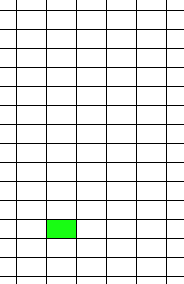
\includegraphics[width=\linewidth,clip=true,trim=0 0 0 100]{CellSelected}
\caption{Poniamoci su una cella}
\end{figure}}

\only<4>{
\begin{figure}
\centering
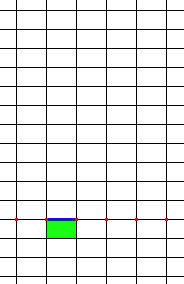
\includegraphics[width=\linewidth,clip=true,trim=0 0 0 100]{Integrating_on_x}
\caption{I contributi della cella ai nodi x}
\end{figure}}

\only<5>{
\begin{figure}
\centering
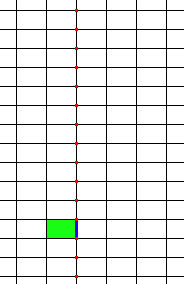
\includegraphics[width=\linewidth,clip=true,trim=0 0 0 100]{Integrating_on_y}
\caption{I contributi della cella ai nodi y}
\end{figure}}

\end{column}
\end{columns}
\end{frame}

%%%%%%%%%%%%%%%%%%%%%%%%%%%%%%%%%%%%%%%%%%%%%%%%%%%%%%%%%%%%%%%%%%%%%%%%%%%%%%%%%%%%%%%%%%%%%%%%%%%%%%%%%%%%%%%%%%%%%%%%%%%%%%%%

\begin{frame}
 \frametitle{Calcolo dell'integrale in forma \emph{log-price}}
 \begin{columns}[c]
%%explanation column
\only<1->{
\begin{column}[t]{.5\linewidth}


In questo caso l'integrale da calcolare è

\begin{equation*}
 \int_{-\infty}^\infty u(t,x+y)\nu(y)dy
\end{equation*}
su una griglia qualunque. Osserviamo che si può uscire dal dominio a causa del termine $x+y$.\\

\only<2->{
In questo caso si realizza un ciclo su tutti i vertici. Selezionato un vertice $i$,}
\only<3->{
si avranno dei nodi di quadratura in direzione $x$ e si quadra su $x_i+z_l$ (in blu), e se la dimensione è due, anche su $y$ lungo $y_i+z_q$ (in verde).} 
\end{column}
}

%%image column
\begin{column}[t]{.5\linewidth}

\only<1>{
\begin{figure}
\centering

\includegraphics[width=\linewidth,clip=true,trim=0 0 0 100]{BaseGrid}
\caption{Una griglia}
\end{figure}}

\only<2>{
\begin{figure}
\centering
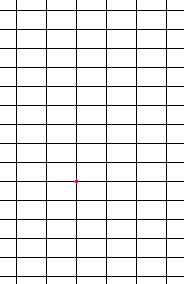
\includegraphics[width=\linewidth,clip=true,trim=0 0 0 100]{VertexSelected}
\caption{Poniamoci su un nodo}
\end{figure}}

\only<3->{
\begin{figure}
\centering
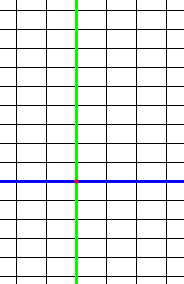
\includegraphics[width=\linewidth,clip=true,trim=0 0 0 100]{LogPrice_X_and_Y_integr}
\caption{Calcolo lungo le direzioni}
\end{figure}}

\end{column}
\end{columns}
 
\end{frame}

%%%%%%%%%%%%%%%%%%%%%%%%%%%%%%%%%%%%%%%%%%%%%%%%%%%%%%%%%%%%%%%%%%%%%%%%%%%%%%%%%%%%%%%%%%%%%%%%%%%%%%%%%%%%%%%%%%%%%%%%%%%%%%%%%%%%%%%%%%%%%%%%%%%%%%%%%%%%%%%%%%%%%%%%%%%%%%%%%%%%%%%%%%%%%%%%%%%%%%%%%%%%%%%%%%%%%%%%%%%%%%%%%%%%%%%%%%%%%%%%%%%%%%%%%%%%%%%%
\section{Struttura del codice}

\begin{frame}
\frametitle{La libreria \textsf{deal.ii}}
\begin{block}{Libreria \textsf{deal.ii}}
Una potente libreria \emph{open source} ad elementi finiti sui quadrilateri. Molto completa e semplice da utilizzare all'inizio, permette di risolvere problemi variazionali fino a 3 dimensioni con poche righe di codice. 
\end{block}
\vspace{0.5cm}
\pause
\begin{block}{Vantaggi}
 \begin{itemize}
  \item Documentazione molto ampia e chiara, a cui si aggiunge la presenza di 51 \emph{tutorial} che illustrano come usare la libreria per problemi pi\`u o meno tipici.
  \item Organizzata in moduli che coprono le diverse aree di un problema ad elementi finiti (\emph{creazione griglie, algebra lineare, output risultati, etc}).
 \end{itemize}
\end{block}
\end{frame}
%%%%%%%%%%%%%%%%%%%%%%%%%%%%%%%%%%%%%%%%%%%%%%%%%%%%%%%%%%%%%%%%%%%%%%%%%%%%%%%%%%%%%%%%%%%%%%%%%%%%%%%%%%%%%%%%%%%%%%%%%%%%%%%%%

\begin{frame}
\frametitle{La nostra implementazione }
 Tre strutture chiave per il problema
 \begin{block}{Classi Opzione}
Rappresentano il problema e gestiscono creazione griglia, assemblaggio sistema e soluzione.
 \end{block}
 \begin{block}{Classi Model}
 I vari modelli utilizzati in finanza sono rappresentati con queste classi, la cui interfaccia è stabilita da una classe base astratta.
 \end{block}
 \begin{block}{Classi Integrali}
  Il calcolo della parte integrale è gestito da queste classi, e le Opzioni salvano un puntatore a un oggetto di questo tipo. 
 \end{block}
 Tutte queste strutture sfruttano il meccanismo dell'ereditarietà al fine di coprire i diversi casi possibili.
\end{frame}

%%%%%%%%%%%%%%%%%%%%%%%%%%%%%%%%%%%%%%%%%%%%%%%%%%%%%%%%%%%%%%%%%%%%%%%%%%%%%%%%%%%%%%%%%%%%%%%%%%%%%%%%%%%%%%%%%%%%%%%%%%%%%%%%%

\begin{frame}[t]
 \frametitle{Le classi Opzione}

 Seguendo la linea di \textsf{deal.ii}, le classi opzione costituiscono il \emph{core} del programma ad elementi finiti. Implementano i vari metodi necessari per la soluzione del problema.\\ Le classi foglia sono quelle effettivamente usate, in quanto implementano tutti i metodi.
 \vspace{1cm}
 \only<1>{\begin{figure}[b!]
  \centering
  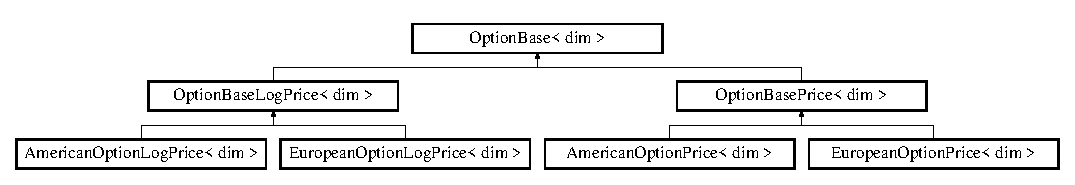
\includegraphics[width=\linewidth]{classOptionBase}
 \caption{Schema delle classi Opzione}
 \end{figure}}
 \vspace{-0.7cm}
 \only<2->{
 \begin{block}{Factory di Opzioni}
  Per facilitare la creazione di opzioni all'utente, è stata creata una \emph{Factory} che permette di creare i vari oggetti \textbf{Opzione} con un'interfaccia comune.
 \end{block}
 }
 \vspace{0.3cm}
 \only<3->{
 \begin{block}{Estensibili}
  L'utente pu\`o sia utilizzare le opzioni gi\`a esistenti, sia crearne delle nuove partendo dal secondo o dal terzo livello di ereditarietà.
 \end{block}
}
\end{frame}



%%%%%%%%%%%%%%%%%%%%%%%%%%%%%%%%%%%%%%%%%%%%%%%%%%%%%%%%%%%%%%%%%%%%%%%%%%%%%%%%%%%%%%%%%%%%%%%%%%%%%%%%%%%%%%%%%%%%%%%%%%%%%%%%%
\begin{frame}[t]
 \frametitle{Le classi Integrale}
 Per calcolare la parte integrale, sono state create una serie di classi. Il secondo livello di ereditarietà distingue fra \emph{price} e \emph{log-price}, mentre le classi foglia implementano quadrature specifiche per i modelli.

 \begin{figure}
  \centering
  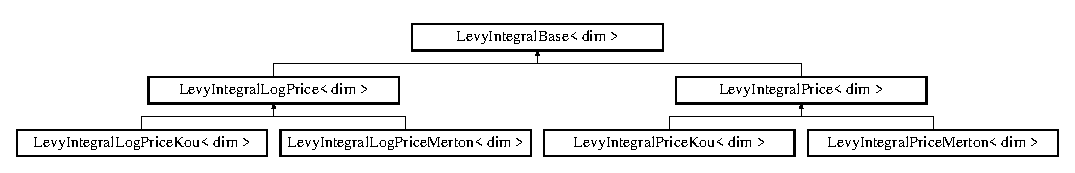
\includegraphics[width=\linewidth]{classLevyIntegralBase}
 \caption{Schema delle classi LevyIntegral}
 \end{figure}
 \pause
 \begin{block}{Generiche}{Le classi base non sono astratte e implementano formule di calcolo generiche (cio\`e, Gauss) per risolvere il problema con modelli qualsiasi.}

 \end{block}
\end{frame}

%%%%%%%%%%%%%%%%%%%%%%%%%%%%%%%%%%%%%%%%%%%%%%%%%%%%%%%%%%%%%%%%%%%%%%%%%%%%%%%%%%%%%%%%%%%%%%%%%%%%%%%%%%%%%%%%%%%%%%%%%%%%%%%%%%%%%%%%%%%%%%%%%%%%%%%%%%%%%%%%%%%%%%%%%%%%%%%%%%%%%%%%%%%%%%%%%%%%%%%%%%%%%%%%%%%%%%%%%%%%%%%%%%%%%%%%%%%%%%%%%%%%%%%%%%%%%%%%%%
\section{Risultati}


\begin{frame}
 \frametitle{Opzioni Europee}
Alcuni esempi di risultati ottenuti: 
\begin{figure}
 \begin{subfigure}{0.48\linewidth}
 \centering
 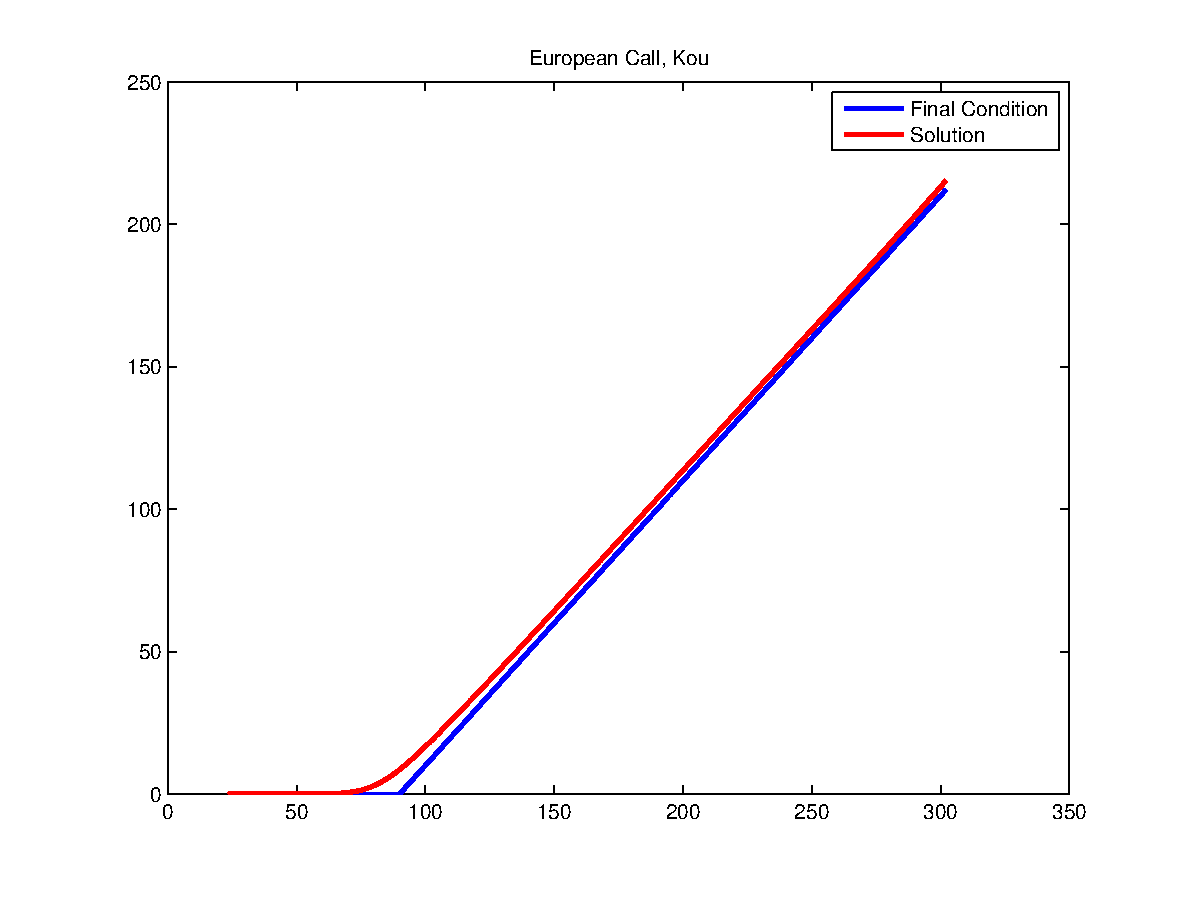
\includegraphics[width=.9\linewidth]{test2-call1dkou}
 \caption{Call europea, modello di Kou}
 \end{subfigure}
 \hfill
 \begin{subfigure}{0.48\linewidth}
  \centering
  \includegraphics[width=0.9\linewidth]{test1-call2dpriceSolution}
  \caption{Call Basket europea, modello di Black\&Scholes}
 \end{subfigure}
 \end{figure}
I risultati, confrontati con la soluzione analitica (nei pochi casi in cui esiste) o con altri \emph{software} di simulazione (differenze finite o Montecarlo), sono corretti.
\end{frame}
%%%%%%%%%%%%%%%%%%%%%%%%%%%%%%%%%%%%%%%%%%%%%%%%%%%%%%%%%%%%%%%%%%%%%%%%%%%%%%%%%%%%%%%%%%%%%%%%%%%%%%%%%%%%%%%%%%%%%%%%%%%%%%%%

\begin{frame}
\frametitle{Opzioni Americane}
Risultati ottenuti nel problema con ostacolo:
\begin{figure}
\begin{subfigure}{0.48\linewidth}
\centering
 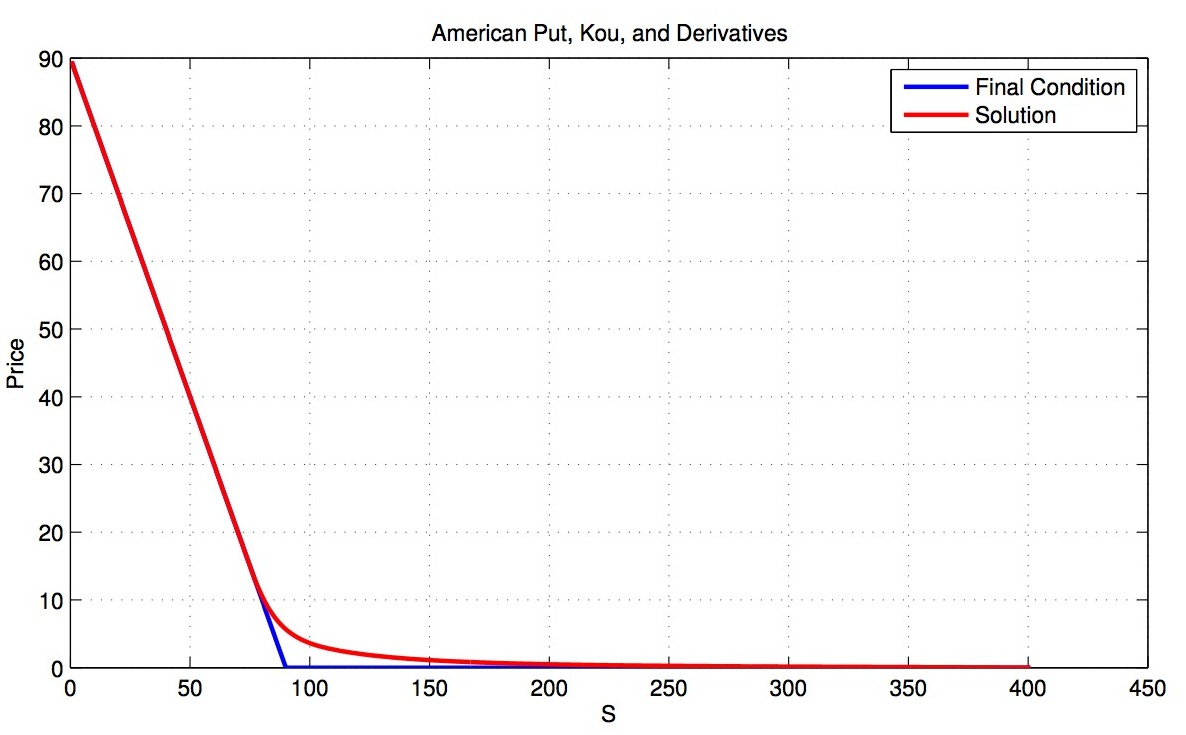
\includegraphics[width=.9\linewidth]{img/us_put.jpg}
 \caption{Put americana, modello di Black\&Scholes}
 \end{subfigure}
 \hfill
 \begin{subfigure}{0.48\linewidth}
  \centering
  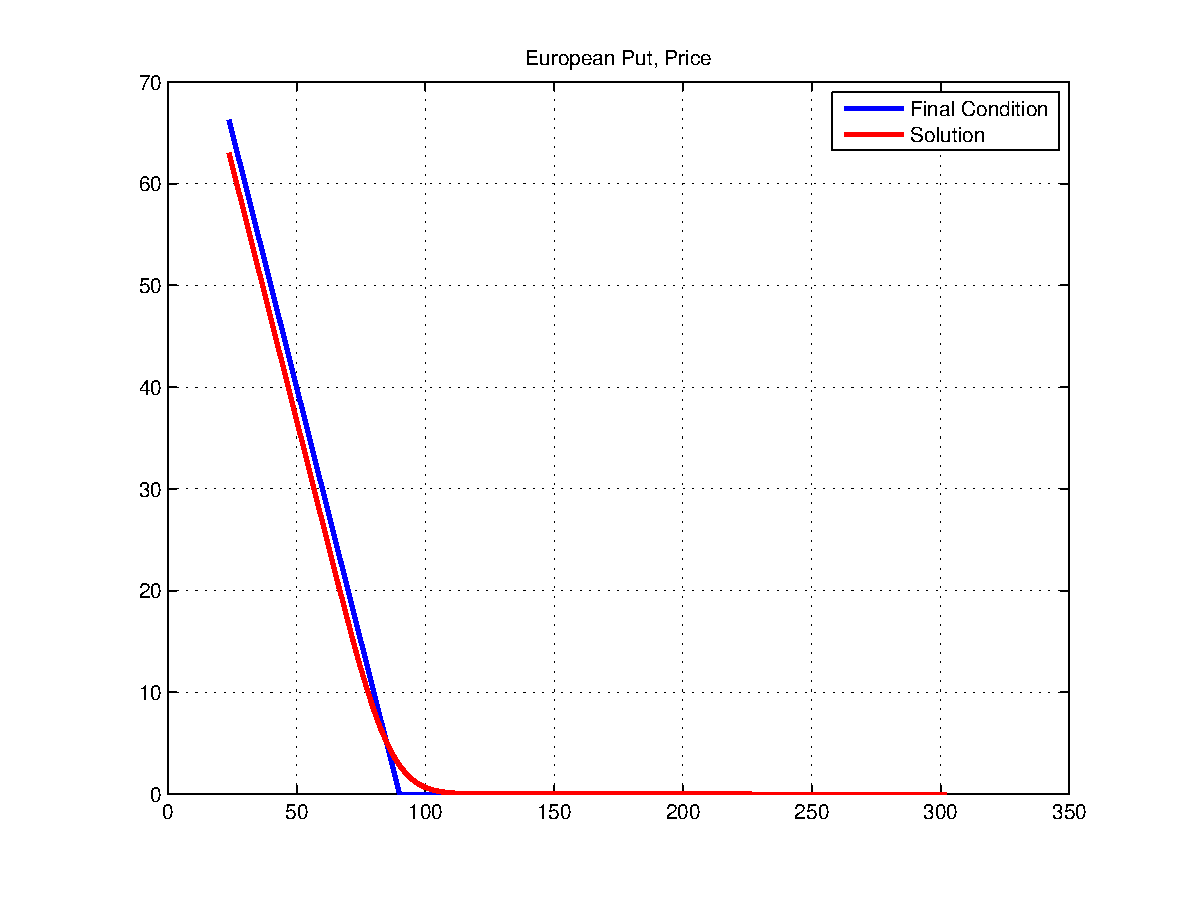
\includegraphics[width=0.9\linewidth]{test1-put1dprice.eps}
  \caption{Put europea, modello di Black\&Scholes}
 \end{subfigure}
 \end{figure}
 Come possiamo notare, il \emph{solver} dell'americana impone che la soluzione stia sempre sopra l'ostacolo, nonostante essa tenda ad andare sotto il \emph{payoff}.
\end{frame}

\begin{frame}[t]
 \frametitle{\emph{Price} v.s \emph{Log-price}}
Con entrambi i metodi si ottengono risultati corretti e soddisfacenti:

%spazio fra le righe!  
\renewcommand{\arraystretch}{1.5}

\only<1>{
\begin{table}
\centering
\begin{tabular}{|p{0.43\linewidth}|p{0.43\linewidth}|}
\hline
\emph{Price} & \emph{LogPrice}\\
\hline
In 1d molto veloce & In 1d mediamente veloce\\
In 2d performance ottime & In 2d lento \\
Non parallelizzabile & Facilmente parallelizzabile (quindi più veloce di \emph{price} 1d con almeno 4 \emph{cores}) \\
No \emph{mesh adapting} in 2d per PIDE & \emph{Mesh adapting} anche in 2d, migliorando le prestazioni\\
Troncamento del dominio può introdurre problemi & Nessun problema troncamento dominio \\
\hline
\end{tabular}
\caption{Confronto fra \emph{Price} e \emph{LogPrice}}
\end{table}}

\only<2>{
\begin{figure}
 \centering
 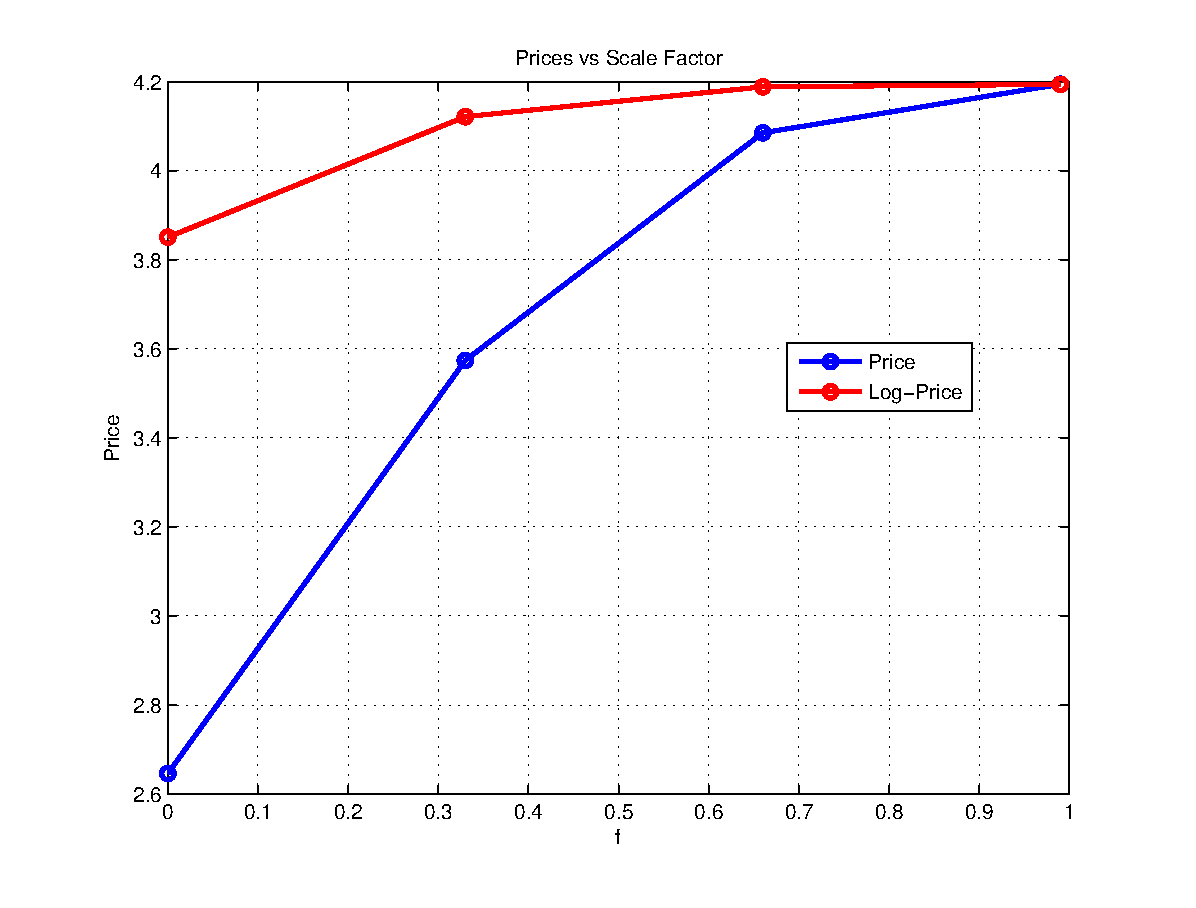
\includegraphics[width=\textwidth,height=0.7\textheight,keepaspectratio]{test2-scalefactor}
\caption{Convergenza del prezzo per una put al variare dello \emph{scaling factor}}
 \end{figure}
}
\end{frame}



%%%%%%%%%%%%%%%%%%%%%%%%%%%%%%%%%%%%%%%%%%%%%%%%%%%%%%%%%%%%%%%%%%%%%%%%%%%%%%%%%%%%%%%%%%%%%%%%%%%%%%%%%%%%%%%%%%%%%%%%%%%%%%%%

\begin{frame}[c]
 \frametitle{\emph{Mesh adaptivity}}
 Utilizzando le funzioni della libreria \textsf{deal.ii}, è facile adattare la griglia:
 \begin{figure}
 \begin{subfigure}{0.48\linewidth}
 \centering
 \only<1>{
 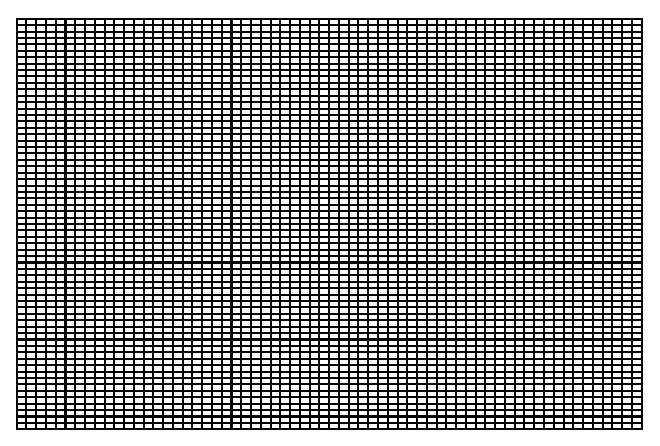
\includegraphics[width=.9\linewidth]{Price1}
 \caption{Griglia iniziale}}
 \only<2->{
 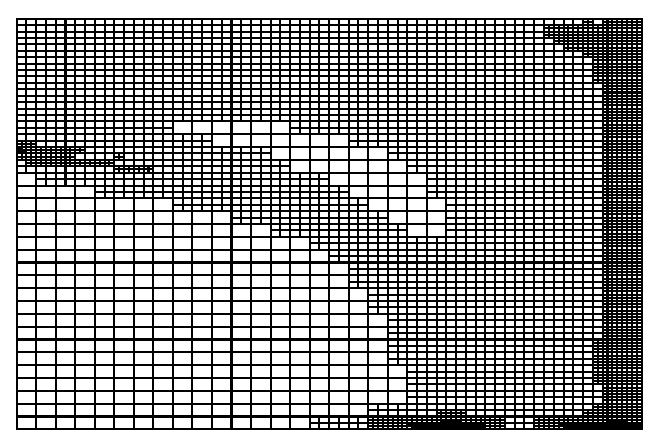
\includegraphics[width=.9\linewidth]{Price3}
 \caption{Griglia adattata}}
 \end{subfigure}
 \hfill
 \begin{subfigure}{0.48\linewidth}
  \centering
  \onslide<2->{
  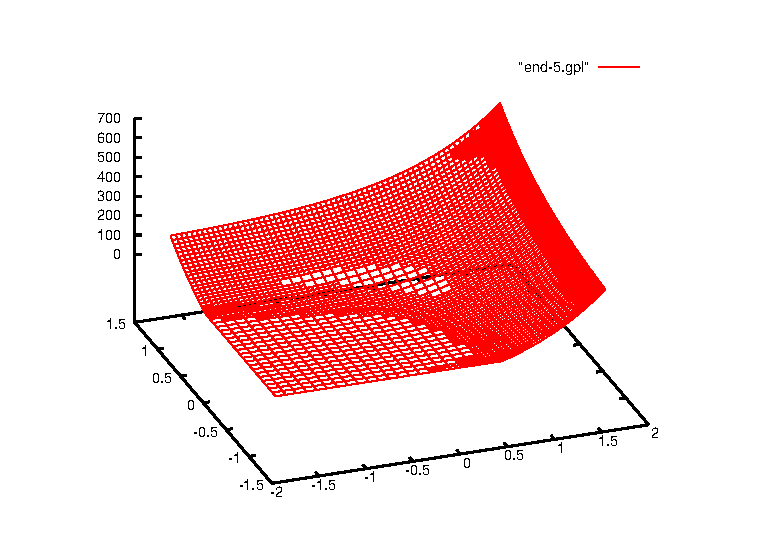
\includegraphics[width=0.9\linewidth]{test5-1}
  \caption{Soluzione con griglia adattata}}
 \end{subfigure}
 \caption{Adattamento di griglia per una Call Europea 2d in forma \emph{LogPrice}}
 \end{figure}
\end{frame}


%%%%%%%%%%%%%%%%%%%%%%%%%%%%%%%%%%%%%%%%%%%%%%%%%%%%%%%%%%%%%%%%%%%%%%%%%%%%%%%%%%%%%%%%%%%%%%%%%%%%%%%%%%%%%%%%%%%%%%%%%%%%%%%%%%%%%%%%%%%%%%%%%%%%%%%%%%%%%%%%%%%%%%%%%%%%%%%%%%%%%%%%%%%%%%%%%%%%%%%%%%%%%%%%%%%%%%%%%%%%%%%%%%%%%%%%%%%%%%%%%%%%%%%%%%%%%%%%%%
\section{Conclusioni}

\begin{frame}
 \frametitle{Bilancio del progetto}
Il programma finale si configura come una piccola ma solida libreria per il \emph{pricing} di derivati finanziari di base, con la possibilit\`a di prezzarne altri facilmente. Inoltre lascia molta libertà all'utente (più trasformazioni, scelta di parametri, \emph{mesh adapting}).
\vspace{0.4cm}
\begin{block}{FEM vs. DFM}
Grazie agli elementi finiti \`e possibile avere un'approssimazione pi\`u pregiata della soluzione, permettendo di calcolare in modo pi\`u preciso anche le derivate.\\
\end{block}
\vspace{0.4cm}
\begin{block}{Prestazioni rispetto ad altri \emph{software}}
Le prestazioni sono migliori se comparate con altri \emph{software}, specialmente nella risoluzione di problemi con ostacolo.
\end{block}
\end{frame}

%%%%%%%%%%%%%%%%%%%%%%%%%%%%%%%%%%%%%%%%%%%%%%%%%%%%%%%%%%%%%%%%%%%%%%%%%%%%%%%%%%%%%%%%%%%%%%%%%%%%%%%%%%%%%%%%%%%%%%%%%%%%%%%

\begin{frame}
 \frametitle{Possibilità di estensioni}
 
 Il progetto, avendo una struttura aperta, si presta molto facilmente ad estensioni. Alcune idee:
 \begin{itemize}[<+->]
  \item aggiunta di altri derivati finanziari simili
  \item aggiunta di altri modelli finanziari
  \item parallelizzazione in memoria distribuita
  \item estensione al caso con tre sottostanti.
 \end{itemize}

 
\end{frame}



%%%%%%%%%%%%%%%%%%%%%%%%%%%%%%%%%%%%%%%%%%%%%%%%%%%%%%%%%%%%%%%%%%%%%%%%%%%%%%%%%%%%%%%%%%%%%%%%%%%%%%%%%%%%%%%%%%%%%%%%%%%%%%%
\begin{frame}[plain]
\centering
 \bf{\LARGE Vi ringraziamo dell'attenzione.}\\
\end{frame}

\end{document}